\chapter{PHÂN TÍCH VÀ THIẾT KẾ HỆ THỐNG}

\section{Kiến trúc hệ thống}

Kiến trúc hệ thống BusGIS được xây dựng dựa trên mô hình ba lớp (Three-tier Architecture) nhằm đảm bảo tính phân tách rõ ràng giữa các thành phần, tối ưu hóa hiệu suất và nâng cao khả năng mở rộng trong tương lai. Sự phân tách này không chỉ giúp cho quá trình bảo trì mã nguồn trở nên thuận tiện mà còn tăng cường mức độ bảo mật cho dữ liệu hệ thống.

Cụ thể, hệ thống bao gồm ba tầng chức năng chính:
\begin{itemize}
    \item \textbf{Tầng Trình diễn (Presentation Layer - Frontend):} Đây là giao diện tương tác trực tiếp với người sử dụng, được xây dựng dựa trên HTML, CSS và framework Bootstrap kết hợp với thư viện LeafletJS. Tầng này chịu trách nhiệm thu nhận yêu cầu của người dùng, chẳng hạn như thao tác tìm kiếm tuyến đường, chọn trạm dừng hoặc thao tác kéo thả trên bản đồ. Sau khi hệ thống xử lý, tầng trình diễn nhận kết quả phản hồi dưới dạng JSON và vẽ lại các lớp bản đồ không gian một cách trực quan. Việc sử dụng LeafletJS giúp giao diện thao tác nhanh chóng, giảm tải băng thông so với việc tải lại toàn bộ trang web.
    \item \textbf{Tầng Xử lý Logic (Business Logic Layer - Backend):} Được phát triển hoàn toàn trên nền tảng Django (Python), tầng này đóng vai trò như bộ não của toàn bộ hệ thống. Nhiệm vụ chính của tầng xử lý logic là tiếp nhận các request từ phía người dùng, tiến hành xử lý nghiệp vụ xác thực, phân quyền và triển khai các thuật toán phân tích không gian phức tạp. Khi có yêu cầu tìm đường hoặc xác định bán kính vùng đệm, Backend sẽ chuyển hóa yêu cầu thành các câu lệnh truy vấn không gian phức hợp, kết nối với cơ sở dữ liệu để lấy kết quả và trả về cho Frontend dưới chuẩn API RESTful.
    \item \textbf{Tầng Dữ liệu (Data Access Layer - Database):} Đóng vai trò cốt lõi trong việc quản lý và duy trì tính toàn vẹn của thông tin. Tầng này sử dụng hệ quản trị cơ sở dữ liệu PostgreSQL kết hợp cùng phần mở rộng PostGIS. Sự kết hợp này mang đến khả năng lưu trữ không chỉ các trường dữ liệu văn bản truyền thống mà còn lưu trữ cấu trúc hình học phức tạp (Point, LineString). PostGIS hỗ trợ việc đánh chỉ mục không gian (Spatial Indexing) bằng cấu trúc R-Tree, giúp các tác vụ truy xuất dữ liệu bản đồ diện rộng được thực thi với tốc độ chỉ tính bằng mili-giây.
\end{itemize}

Sự kết hợp đồng bộ giữa ba tầng kiến trúc trên đã tạo ra một hệ thống WebGIS hoàn chỉnh, hoạt động xuyên suốt từ bước thu nhận yêu cầu của người dùng đến lúc truy xuất, tính toán số liệu và trả về kết quả đồ họa trên giao diện.

\section{Luồng dữ liệu (Data Flow / Pipeline)}

Quá trình luân chuyển dữ liệu bên trong hệ thống BusGIS được thiết kế một cách khoa học nhằm kiểm soát chặt chẽ trạng thái vòng đời của thông tin, từ giai đoạn thu thập ban đầu cho đến khi được biểu diễn trực quan trên bản đồ. Luồng xử lý dữ liệu được chia thành nhiều quy trình nối tiếp nhau, đảm bảo dữ liệu luôn đạt tiêu chuẩn đầu vào của hệ quản trị cơ sở dữ liệu.

Quy trình luân chuyển dữ liệu được thực hiện qua các bước chi tiết sau:
\begin{itemize}
    \item \textbf{Thu thập và Trích xuất dữ liệu thô:} Dữ liệu ban đầu về các tuyến xe buýt và điểm dừng được trích xuất từ cộng đồng bản đồ mở OpenStreetMap bằng cú pháp truy vấn Overpass QL. Dữ liệu trả về thường ở định dạng JSON dạng thô, mang theo rất nhiều thẻ (tags) dư thừa không cần thiết cho ứng dụng.
    \item \textbf{Tiền xử lý và Làm sạch (Data Cleansing):} Tại giai đoạn này, các tập lệnh Python (Scripts) sẽ duyệt qua bộ dữ liệu thô. Quá trình làm sạch tập trung vào việc loại bỏ các node không chứa thông tin quan trọng, chuẩn hóa tên tuyến xe, xử lý các ký tự đặc biệt trong địa chỉ trạm dừng và định dạng lại cấu trúc mảng tọa độ. Dữ liệu sau đó được định hình lại theo chuẩn GeoJSON với cấu trúc phân cấp thống nhất.
    \item \textbf{Chuyển đổi và Lưu trữ (Transform \& Load):} Từ tập dữ liệu GeoJSON đã làm sạch, Django ORM tiến hành chuyển đổi các cặp kinh độ, vĩ độ thành đối tượng hình học dạng điểm (Point) và chuỗi đường (LineString) tuân thủ hệ tọa độ WGS84 (SRID 4326). Dữ liệu này sau đó được ánh xạ trực tiếp vào các bảng quan hệ trong PostGIS, đồng thời tạo ra các mối liên kết khóa ngoại (Foreign Keys) giữa bảng Tuyến, bảng Trạm và bảng trung gian (RouteStop).
    \item \textbf{Truy vấn và Phân tích (Query \& Analysis):} Khi có yêu cầu tương tác từ người dùng (như nhấn chọn xem chi tiết tuyến), hệ thống thực hiện lệnh truy vấn SQL thông qua Django ORM. Dữ liệu được trích xuất từ cơ sở dữ liệu, đi qua các bộ lọc và hàm phân tích không gian (nếu có), sau đó đóng gói thành định dạng JSON.
    \item \textbf{Hiển thị trực quan (Visualization):} Frontend nhận gói dữ liệu JSON từ Backend, sử dụng các hàm API của LeafletJS để vẽ đối tượng lên không gian bản đồ. Các điểm (Markers) biểu thị cho trạm dừng, các đường gấp khúc (Polylines) biểu thị cho lộ trình di chuyển. Mỗi đối tượng đều được đính kèm các popup hiển thị thông tin chi tiết.
\end{itemize}

\section{Thiết kế cơ sở dữ liệu}

Cơ sở dữ liệu của BusGIS được thiết kế đảm bảo các chuẩn mực chuẩn hóa, giảm thiểu tối đa hiện tượng dư thừa dữ liệu và hỗ trợ đắc lực cho các liên kết không gian. 

\begin{figure}[H]
    \centering
    
\includegraphics[width=\textwidth]{images/image1.png}
    \caption{Mô hình thực thể kết nối (ERD) tổng quan}
\end{figure}

Dữ liệu được chia thành các bảng chính bao gồm:
\begin{itemize}
    \item \textbf{Bảng BusRoute:} Lưu trữ thông tin chi tiết của tuyến xe như số hiệu tuyến, tên tuyến, điểm đầu, điểm cuối, thời gian hoạt động, giá vé và màu sắc hiển thị trên bản đồ.
    \item \textbf{Bảng BusStop:} Lưu trữ vị trí không gian của các trạm xe buýt. Điểm nổi bật là trường vị trí được cấu hình kiểu hình học \texttt{Point(Lon, Lat)} để truy vấn khoảng cách. Ngoài ra còn lưu thông tin mã trạm, tên trạm, địa chỉ và các tiện ích đi kèm (mái che, ghế ngồi).
    \item \textbf{Bảng RouteStop (Trung gian):} Quản lý mối quan hệ nhiều - nhiều giữa Tuyến và Trạm. Bảng này không chỉ liên kết khóa ngoại mà còn lưu trữ trường Thứ tự (Order) nhằm xác định hướng di chuyển chính xác của tuyến xe.
    \item \textbf{Bảng User và UserProfile:} Quản lý tài khoản người dùng, lưu trữ thông tin xác thực, phân quyền hệ thống (User, Staff, Admin) và các thông tin liên hệ.
    \item \textbf{Bảng Review:} Cho phép người dùng đánh giá và phản hồi về tuyến xe buýt hoặc trạm dừng, bao gồm điểm số đánh giá và nội dung nhận xét.
\end{itemize}

\section{Thiết kế chức năng (Use Case)}

Hệ thống BusGIS cung cấp đa dạng các chức năng đáp ứng nhu cầu cho hai nhóm đối tượng chính: Người dùng khách (Guest/User) và Quản trị viên (Admin/Staff).

\begin{figure}[H]
    \centering
    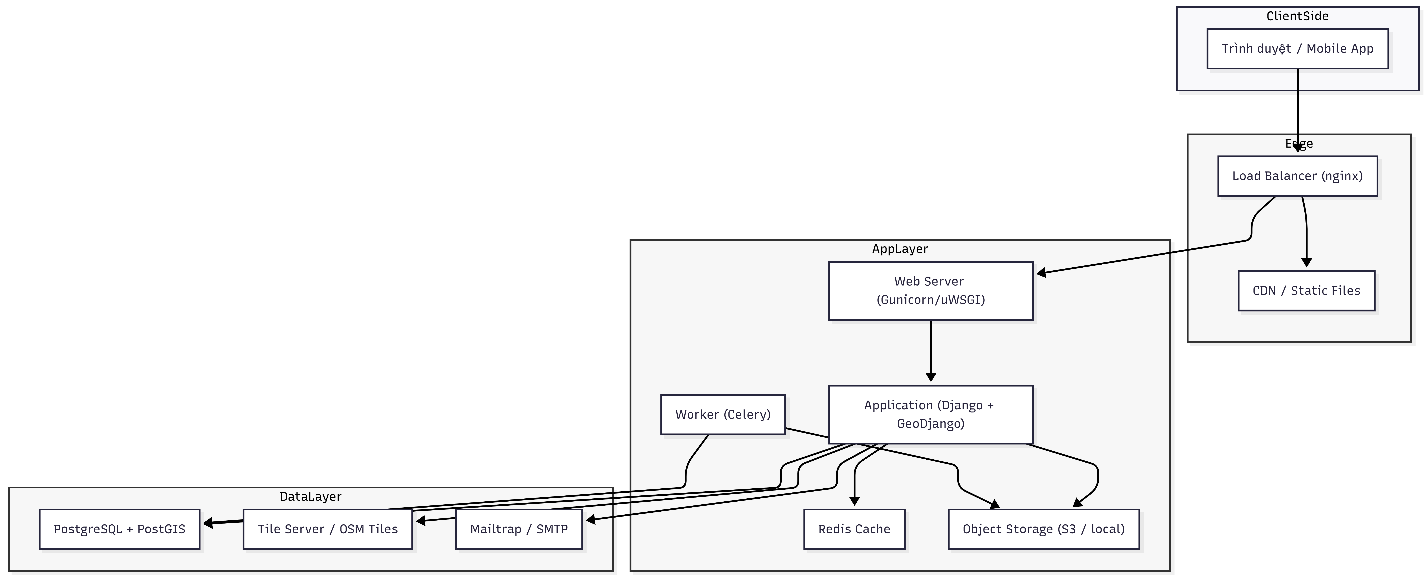
\includegraphics[width=\textwidth]{images/image2.png}
    \caption{Sơ đồ Use Case tổng quát hệ thống}
\end{figure}

Các chức năng chính được phân chia theo từng vai trò như sau:
\begin{itemize}
    \item \textbf{Nhóm chức năng dành cho Người dùng:}
    \begin{itemize}
        \item Tra cứu tuyến xe buýt, xem chi tiết đường đi, điểm đầu cuối, giá vé.
        \item Tìm kiếm trạm dừng, xác định vị trí trạm trên bản đồ và tiện ích tại trạm.
        \item Đăng ký tài khoản, đăng nhập và quản lý thông tin hồ sơ cá nhân.
        \item Sử dụng các công cụ GIS nâng cao: Tìm tuyến đường theo tọa độ hiện tại, tìm trạm dừng trong phạm vi bán kính cho trước.
        \item Gửi đánh giá, nhận xét trải nghiệm sử dụng đối với từng tuyến xe hoặc trạm dừng.
    \end{itemize}
    
    \item \textbf{Nhóm chức năng dành cho Quản trị viên:}
    \begin{itemize}
        \item Quản trị toàn diện mạng lưới dữ liệu xe buýt (Thêm, Sửa, Xóa mềm đối với Tuyến xe và Trạm dừng).
        \item Import và Export dữ liệu hàng loạt từ các định dạng Excel, hỗ trợ cập nhật thông tin nhanh chóng.
        \item Quản lý tài khoản người dùng, theo dõi trạng thái hoạt động và phân quyền nhân viên.
        \item Theo dõi và kiểm duyệt các đánh giá (Reviews) từ người dùng đối với các dịch vụ.
        \item Truy cập bảng thống kê trực quan (Dashboard) hiển thị tổng quan số lượng tuyến, trạm và lưu lượng tương tác của hệ thống.
    \end{itemize}
\end{itemize}

Để làm rõ chi tiết nghiệp vụ thao tác, các quy trình cốt lõi được biểu diễn thông qua Sơ đồ Tuần tự (Sequence Diagram) và Sơ đồ Hoạt động (Activity Diagram).

\begin{figure}[H]
    \centering
    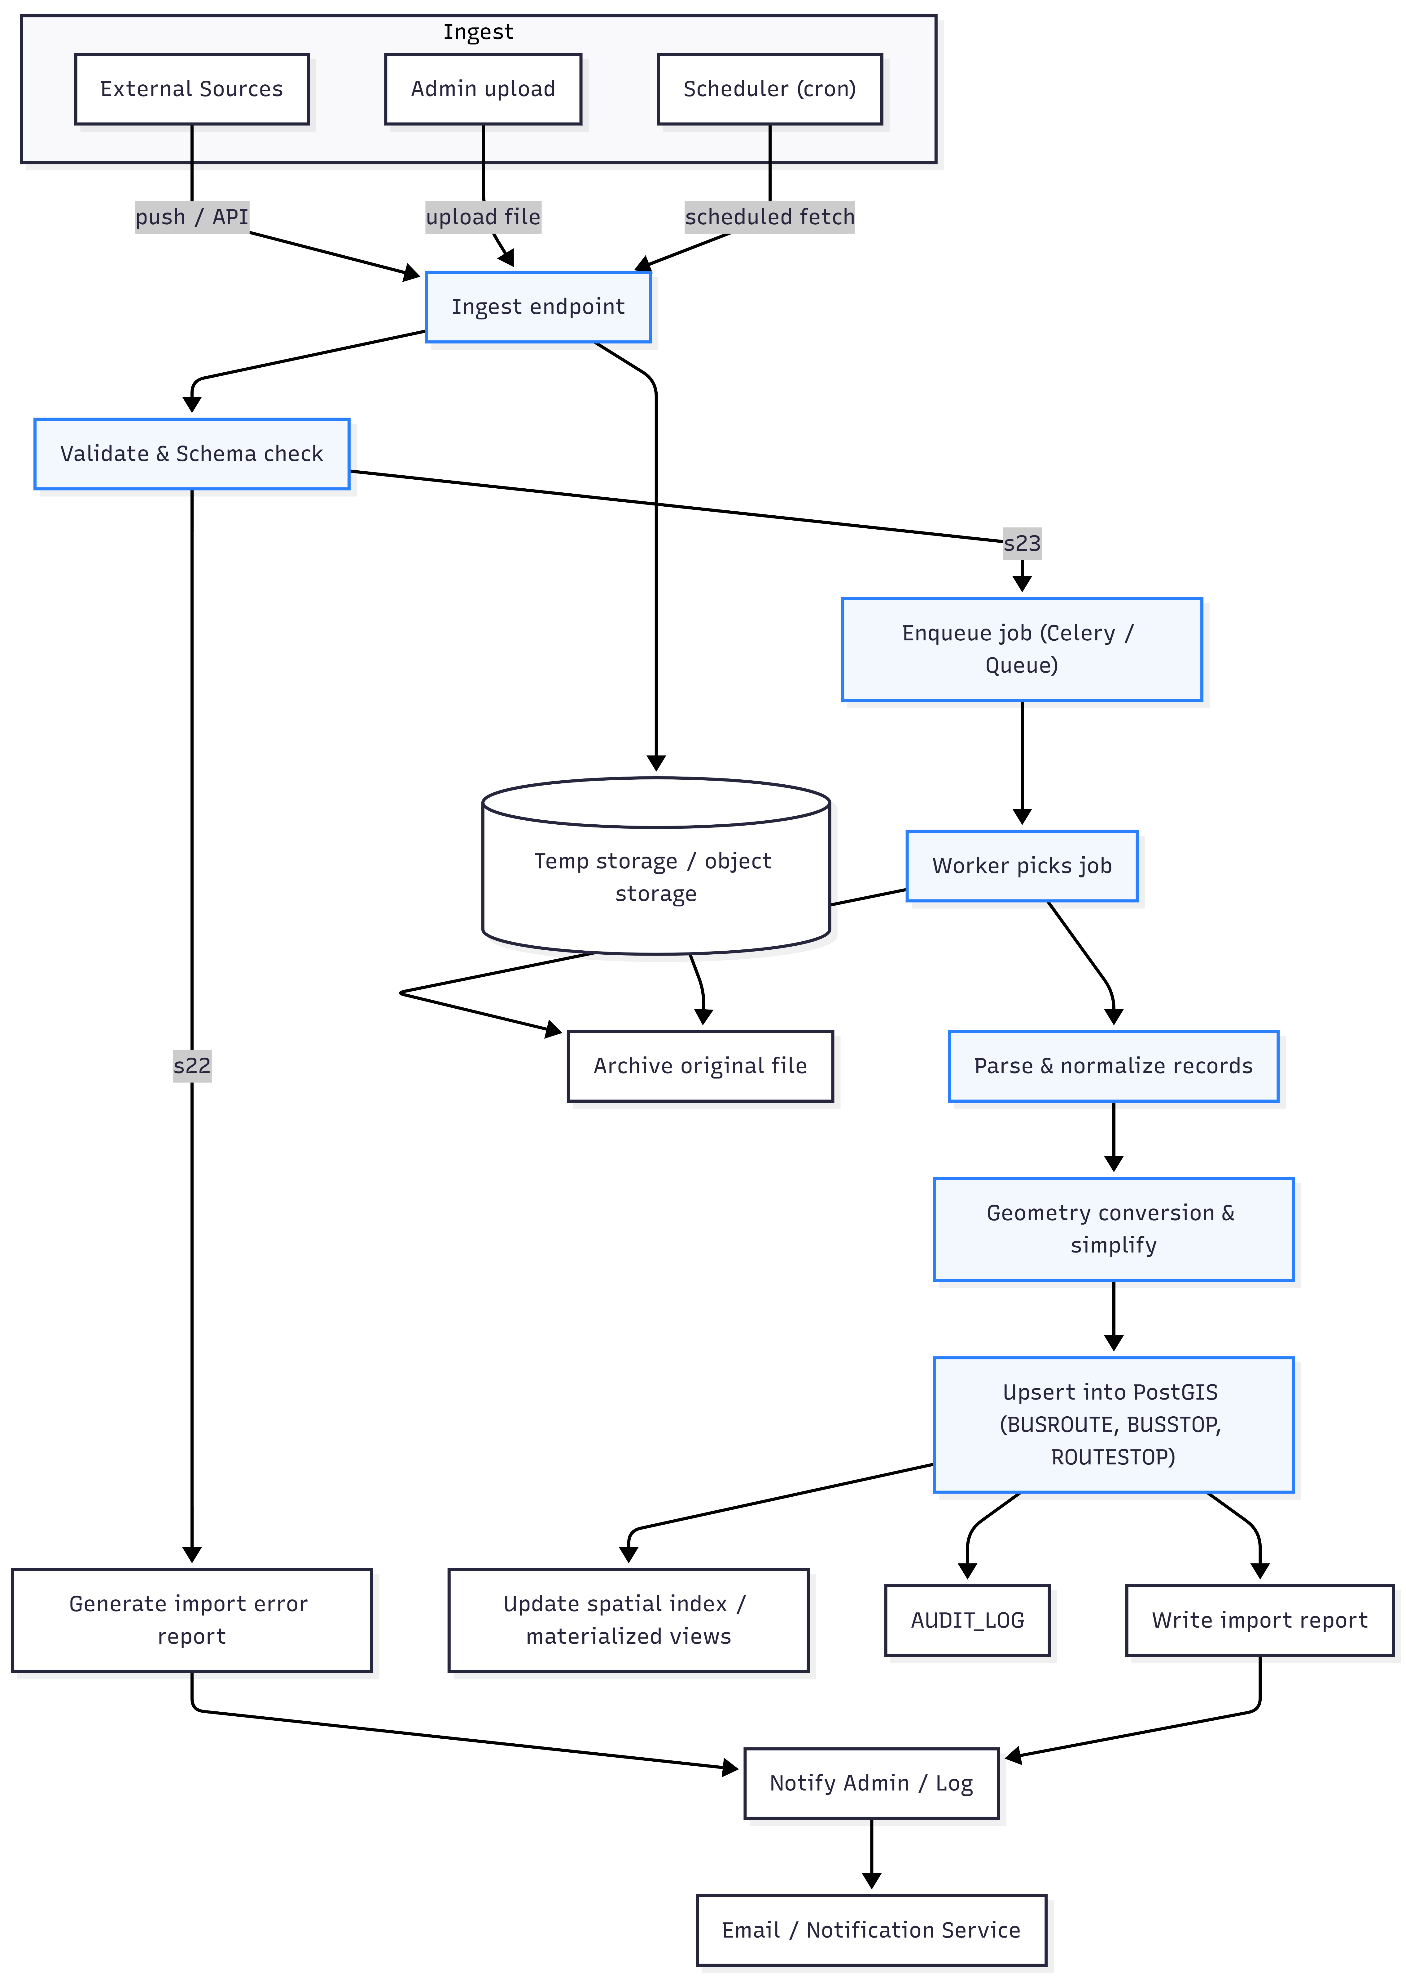
\includegraphics[width=\textwidth]{images/image3.png}
    \caption{Sơ đồ hoạt động quy trình tìm kiếm và định tuyến}
\end{figure}

Sơ đồ trên minh họa quá trình người dùng nhập điểm bắt đầu và kết thúc, hệ thống sẽ giao tiếp với máy chủ PostGIS để tính toán thuật toán khoảng cách và phản hồi danh sách các tuyến phù hợp để biểu diễn lên bản đồ trực quan.
